\newpage
\section{先行研究}
本章では,本研究で開発したロボットのベースとなった機体を先行研究を用いて述べ,それぞれの実験結果とそこから得られた知見をまとめる.

\subsection{柔軟外皮装着型魚ロボット}
先行研究で開発された機体を図\ref{fig:robot_sen}に,構造を図\ref{fig:kouzou_sen}に示す.図は魚型ロボットに柔軟外皮を取り付けたものであり,水中に沈めること及び水中での姿勢維持を目的として,外皮を固定す
る防水リングにおもりが取り付けてある.おもりの重さは頭部と尾びれ部分でそれぞれ296 g,150 gである.本機体は全長477 mm,重さ1080 g,おもりを含めた重さが1526 g
となっている.本機体は頭部と胴体部の大きく二つに分けることができる.

\subsubsection{頭部}
本機体の頭部には,DC モータ( タミヤ社,AO-8033),サーボモータ(Tower Pro 社,MG92B)二つ,マイコン(M5Stack Technology 社,M5STACK-K051),モータ用Lipo バッ
テリ(Hyperion 社,G5 50Cmax 7.4 V-240 mAh),マイコン用Lipo バッテリ(DATA POWERTECHNOLOGY 社,DTP502535),スイッチが入っている.モータは頭部に収まるものの中
でなるべくトルクの強いものを選んだ.また,上に挙げたスイッチ以外の部品はすべて頭部の外殻ではなく内側のふたに取り付けられている.

\begin{figure}[htbp]
    \centering
    \begin{tabular}{cc}
     \begin{minipage}[b]{0.45\linewidth}
        \centering
        \setPicture{zenrarobot.jpg}
        \subcaption{外皮未装着時}
        \label{fig:gaihi_sen}
     \end{minipage}
     \hspace{0.05\linewidth}
     \begin{minipage}[b]{0.45\linewidth}
        \centering
        \setPicture{fishrobot.jpg}
        \subcaption{外皮装着時}
        \label{fig:migaihi_sen}
     \end{minipage}
    \end{tabular}
    \caption{柔軟外皮装着型の魚ロボット}
    \label{fig:robot_sen}
\end{figure}
\begin{figure}[htbp]
    \centering
    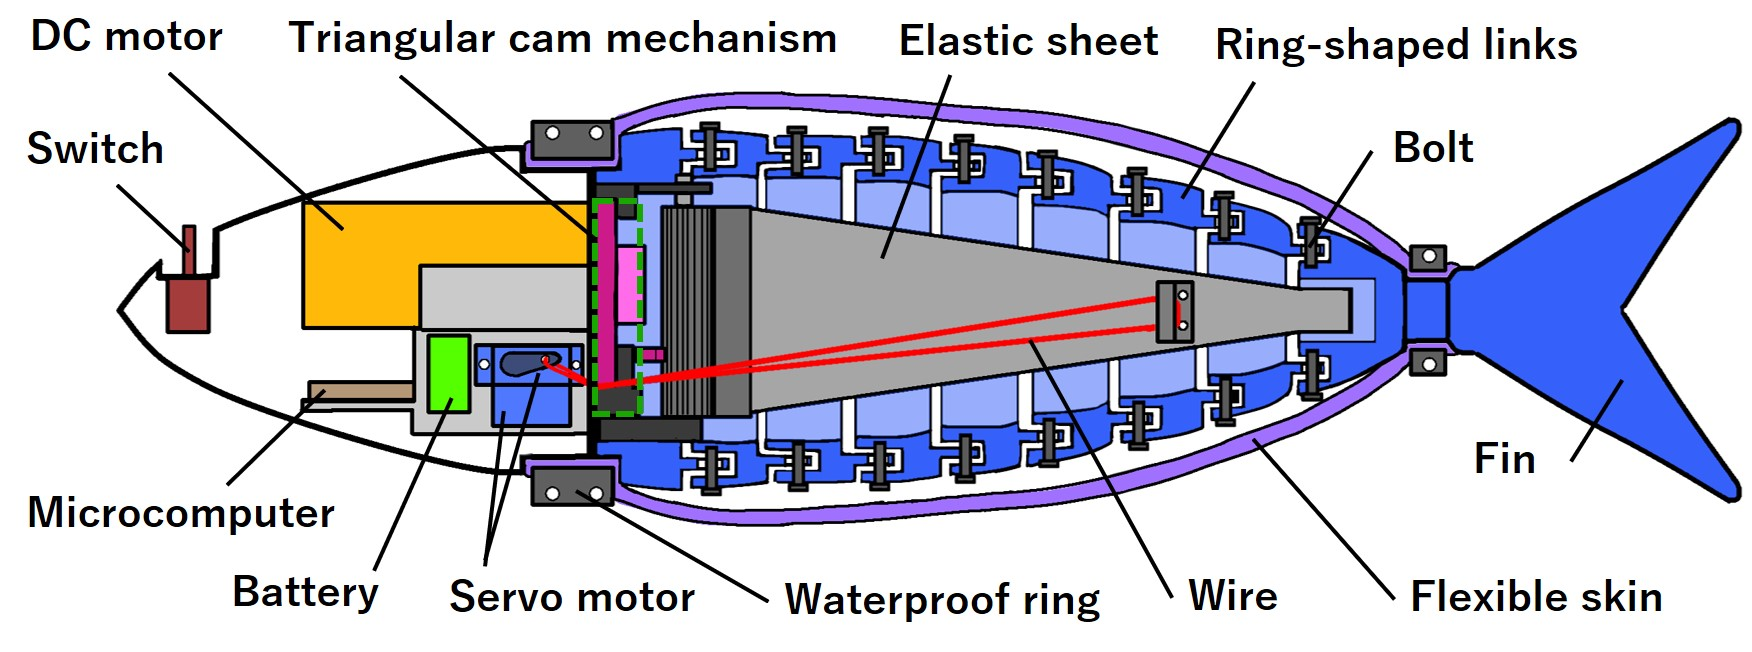
\includegraphics[width=0.6\linewidth]{/Users/watanabe_shouta/2024_graduation_thesis/picture/mosikizu.jpg}
    \caption{ロボットの構造}
    \label{fig:kouzou_sen}
\end{figure}
\begin{figure}[t]
    \centering
    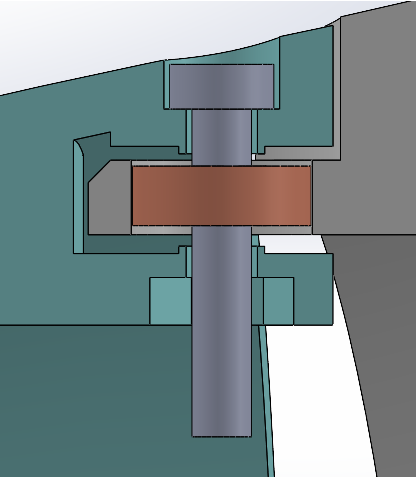
\includegraphics[width=0.3\linewidth]{/Users/watanabe_shouta/2024_graduation_thesis/picture/link.png}
    \caption{関節の構造}
    \label{fig:kansetu}
\end{figure}

\subsubsection{胴体部}
胴体部は屈曲可能な8関節9リンク構造になっており,リンクの接続部は図\ref{fig:kansetu}のようにベアリング(内径3 mm)とボルト(M2)で接続されている.また,すべてのリンクで合計
$90\:^\circ$曲げるため一関節あたり$11.25\:^\circ$曲がるよう設計されている.$90\:^\circ$という値は,実際のハマチの動く様子から決定している.なお,各リンクには機体を
水中に沈めるために板おもり(22 g)を合計10 枚張り付けてある.次に,飛び移り座屈に用いる弾性体について記す.ここでの弾性体とは外力により曲がる薄い板のことを指す.先行研究
では0.2 mm厚のステンレス(岩田製作所,SUS02)に加え,弾性を強めるために1 mm厚のポリプロピレン(セイワ・プロ社,23-589)を貼り合わせたものを使用している.

\subsection{実験条件}


